% (c) 2012 - 2014 Dimitrios Vrettos - d.vrettos@gmail.com
% (c) 2014 Claudio Carboncini - claudio.carboncini@gmail.com
\chapter{Numeri interi relativi}
\section{I numeri che precedono lo zero}

Con i numeri naturali non sempre è possibile eseguire l'operazione di sottrazione. In particolare,
non è possibile sottrarre un numero più grande da un numero più piccolo, per esempio~$5-12$. Tuttavia
ci sono situazioni in cui una sottrazione di questo tipo deve essere eseguita.

Per esempio, è possibile acquistare un'auto di \officialeuro~$12\,000$ pur avendo soltanto risparmi in banca di soli
\officialeuro~$5\,000$. In questo caso si tratta di togliere dai \officialeuro~$5\,000$ i \officialeuro~$12\,000$ che servono per acquistare
l'auto: materialmente non è possibile e si ricorre a un prestito.

Pensiamo ad una comunicazione dei meteorologi relativa alle previsioni del tempo: <<domani la temperatura,
a causa di una perturbazione proveniente dai paesi nordici, potrebbe subire un drastico calo e scendere anche di~10 gradi>>. Riflettiamo: se oggi la temperatura è di~9 gradi, come possiamo esprimere numericamente la temperatura
prevista per domani? Alcuni diranno: <<il liquido contenuto nel termometro si posizionerà al di sotto dello zero>>,
altri <<domani la temperatura sarà di un grado sotto lo zero>> e
altri ancora <<la temperatura sarà di~$-1$ grado>>.

\begin{wrapfloat}{figure}{r}{0pt}
 % (c) 2012 Dimitrios Vrettos - d.vrettos@gmail.com
% Monte Everest e Fossa delle Marianne
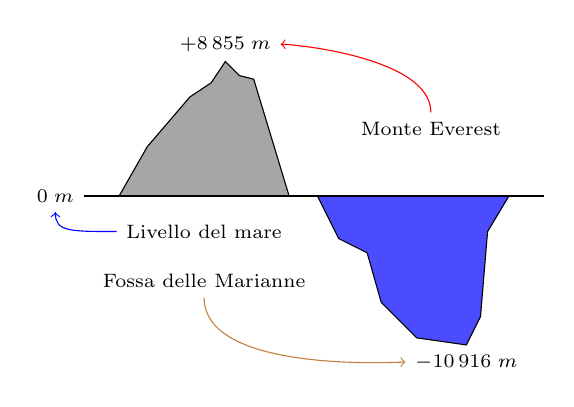
\begin{tikzpicture}[scale=.9]
  % Disegna Everest
  \filldraw[fill=gray!70, draw=black] (0,0)-- (4mm,7mm)-- (10mm,14mm)--(13mm,16mm)-- (15mm,19mm)--(17mm,17mm)--%
	    (19mm,16.5mm)--(24mm,0);
  % Disegna Fossa delle Marianne
  \filldraw[fill=blue!70, draw=black](28mm,0)--(31mm,-6mm)--(35mm,-8mm)--(37mm,-15mm)--(42mm,-20mm)-- (49mm,-21mm)--%
	    (51mm, -17mm)--(52mm, -5mm)--(55mm,0);
  % Disegna il livello del mare 
  \draw[thick] (-5mm,0) -- (60mm,0);

  \begin{scope}[font=\scriptsize]
    % Posiziona altezze
    \node[left] (0)at (-5mm,0) {$0\;\unit{m}$};
    \node [above](everest) at (15mm,19mm) {$+8\,855\;\unit{m}$};
    \node [below](marianne) at (49mm,-21mm) {$-10\,916\;\unit{m}$};
    % Posiziona etichette
    \node (testo1) at (44mm,9.5mm) {Monte Everest};
    \node (testo2) at (12mm,-5mm) {Livello  del mare};
    \node (testo3) at (12mm,-12mm) {Fossa delle Marianne};
  \end{scope}
  % Disegna frecce
  \draw[<-,red ] (everest) .. controls +(right:10mm) and +(up:10mm) .. node[]{} (testo1);
  \draw[<-, blue](0)..controls +(down:5mm) and +(left:19mm)..node[]{} (testo2);
  \draw[<-, brown](marianne)..controls +(left:10mm) and +(down:13mm)..node[]{} (testo3);

\end{tikzpicture}

 \caption{Il monte Everest e la fossa delle Marianne.}
 \label{fig:everest}
\end{wrapfloat}

Leggiamo nel testo di geografia: <<Il punto più profondo della Terra si trova nella fossa delle Marianne; esso
supera di~$2\,061$ metri l'altezza del monte Everest e si trova a~$10\,916$ metri sotto il livello del mare>>.
Se attribuiamo al livello del mare l'altitudine 0, allora potremmo esprimere la profondità della Fossa con il
numero~$-10\,916$ e l'altezza del monte Everest con il numero~$+8\,855$ (figura \ref{fig:everest}).

Per rappresentare le grandezze che hanno due sensi, come temperature, crediti e i debiti, latitudine nord e sud,
altezze sopra il livello del mare e profondità marine i numeri naturali non bastano. I matematici in queste
situazioni usano i \emph{numeri interi relativi} che si scrivono utilizzando gli stessi numeri naturali ma preceduti
dal segno~``$+$'' se sono numeri maggiori di~0 e dal segno~``$-$'' se sono numeri minori di~0. L'insieme di questi numeri
si costruisce raddoppiando i numeri naturali~$\insN$ e facendo precedere ciascun numero dal segno~``$+$'' o~``$-$'',
ad eccezione dello~0, al quale non si attribuisce segno.

\[ \insZ=\lbrace\ldots\text{,~}-5\text{,~}-4\text{,~}-3\text{,~}-2\text{,~}-1\text{,~}0\text{,~}+1\text{,~}+2\text{,~}+3\text{,~}+4\text{,~}+5\text{,~}\ldots\rbrace \]
\pagebreak

\section{I numeri relativi e la retta}

I numeri relativi possono essere rappresentati su una retta. Disegniamo una retta, su di essa prendiamo
un punto di riferimento al quale associamo il numero zero, il verso di percorrenza da sinistra verso destra,
un segmento~$AB$ come un'unità di misura. Riportiamo questa unità di misura più volte partendo da zero e
procedendo nel verso stabilito aggiungiamo ogni volta uno: ai punti trovati associamo gli interi positivi.
Ripetiamo l'operazione partendo dallo zero, ma con il verso di percorrenza a sinistra: ai punti trovati associamo
gli interi negativi.

\begin{center}
 % (c) 2012 Dimitrios Vrettos - d.vrettos@gmail.com
% La retta degli interi
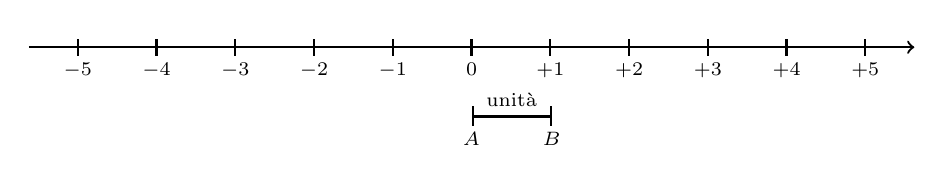
\begin{tikzpicture}
\begin{scope}[thick,font=\scriptsize]
  \draw[->] (-160pt,0)  - -  (160pt,0) node[above]{$\insZ$};	
    \foreach \n in {-5,-4,...,0}{%
      \draw (\n,-3pt) -- (\n,3pt)   node [below=5pt] {$\n$};		
    }

    \foreach \m in {1,2,...,5}{%
      \draw (\m,-3pt) -- (\m,3pt) node [below=5pt]{+$\m$};
    }
  
    \draw[|-|](0,-25pt) node[below=2pt] {$A$} -- node[above] {unit\`a} (29pt,-25pt) node[below=2pt] {$B$};
\end{scope}

\end{tikzpicture}

\end{center}

Possiamo interpretare questi numeri come il numero di passi da fare sulla retta, partendo dallo zero verso
destra se il segno è positivo, verso sinistra se il segno è negativo.

L'insieme dei numeri relativi si indica con il simbolo~$\insZ$. In particolare, l'insieme dei soli numeri interi relativi
con segno positivo si indica con il simbolo~$\insZ^+$ e
l'insieme dei soli numeri interi negativi si indica con il simbolo~$\insZ^-$.

\begin{definizione}
 Due numeri relativi si dicono \emph{concordi}, se hanno lo stesso segno; si dicono \emph{discordi} se hanno
 segni opposti.
\end{definizione}

\begin{exrig}
 \begin{esempio}
 Concordi-discordi.
 \begin{itemize*}
\item $+3$ e~$+5$ sono concordi;
\item $+3$ e~$-5$ sono discordi;
\item $-5$ e~$-2$ sono concordi.
 \end{itemize*}
\end{esempio}
\end{exrig}

\begin{definizione}\label{def:valass}
Il \emph{valore assoluto} di un numero relativo è il numero senza il segno; quindi un numero naturale.
\end{definizione}

Il valore assoluto si indica inserendo il numero relativo tra due barre verticali~$\valass{*}$. In linguaggio
matematico:

\[ \valass{a}=a\text{~~se }a\ge0\text{,}\qquad \valass{a}=-a\text{~~se }a<0.\]

\begin{exrig}
 \begin{esempio}
 Valore assoluto.
 \begin{itemize*}
 \item $\valass{+2}=2$;
 \item $\valass{-5}=5$;
 \item $\valass{-73}=73$;
 \item $\valass{+13}=13$.
 \end{itemize*}
 \end{esempio}
\end{exrig}

\begin{definizione}
 Due numeri interi relativi sono \emph{uguali} se hanno lo stesso segno e lo stesso valore assoluto;
 si dicono \emph{opposti} se hanno lo stesso valore assoluto ma segni diversi.
\end{definizione}

Sono numeri opposti~$+3$ e~$-3$;~$+5$ e~$-5$;~$+19$ e~$-19$.

\osservazione Per indicare un numero positivo è possibile scrivere il numero senza il segno~``$+$''.
Per esempio si può scrivere indifferentemente~$+1$ o~1,~$+12$ o semplicemente~12.

\section{Confronto di numeri relativi}

Dati due numeri interi relativi quello più grande è quello che sulla retta è rappresentato più a destra.
In particolare:
 \begin{enumeratea}
 \item ogni numero intero positivo è maggiore di~0 e di ogni numero negativo;
 \item tra due numeri positivi il più grande è quello che ha valore assoluto maggiore;
 \item ogni numero negativo è minore di~0 e di ogni numero positivo;
 \item tra due numeri negativi il più grande è quello che ha valore assoluto minore;
 \item 0 è minore di ogni numero positivo e maggiore di ogni numero negativo.
 \end{enumeratea}

In maniera analoga a quanto visto per i numeri naturali $\insN$, anche per i numeri relativi $\insZ$ si possono usare i simboli di disuguaglianza: per indicare, ad esempio, che un numero è maggiore di un altro si usa separare i due numeri con il
simbolo~``$>$''; per indicare che il primo è minore del secondo si usa mettere tra i due numeri il simbolo~``$<$''.

\begin{exrig}
 \begin{esempio}
 Confronto di numeri relativi.
 \begin{itemize*}
 \item $+4>+2$: i numeri sono positivi, il maggiore è~$+4$ perché ha valore assoluto maggiore;
 \item $-1>-3$: i due numeri sono negativi, il maggiore è~$-1$ perché ha valore assoluto minore;
 \item $-2<+4$: il numero negativo è minore del numero positivo;
 \item $+4>0$: ogni numero positivo è maggiore di~0;
 \item $-2<0$: ogni numero negativo è minore di~0.
 \end{itemize*}
 \end{esempio}
\end{exrig}

Usando la rappresentazione dei numeri sulla retta l'ordinamento risulta più facile da verificare:
il verso di percorrenza della retta (la freccia) indica la direzione nella quale i numeri crescono.

\vspazio\ovalbox{\risolvii \ref{ese:2.1}, \ref{ese:2.2}, \ref{ese:2.3}, \ref{ese:2.4}}

\section{Le operazioni con i numeri relativi}

Con i numeri relativi è sempre possibile eseguire le addizioni, le moltiplicazioni e le sottrazioni.
Questo significa che se si addizionano, si sottraggono o si moltiplicano due numeri relativi il risultato si
trova sempre nella retta dei numeri relativi.

\subsection{Addizione}

Osserviamo prima di tutto che il simbolo di addizione~$(+)$ è lo stesso che si usa per indicare il segno dei numeri
positivi, pertanto occorre prestare attenzione quando si incontra il segno~``$+$'' al significato che esso ha.
Almeno all'inizio è bene usare una scrittura del tipo~$(+2)+(+5)$ per indicare la somma tra i numeri~$+2$ e~$+5$.

L'addizione di due numeri relativi si esegue in due modi diversi a seconda che gli addendi siano concordi o discordi.

La \emph{somma di due numeri relativi concordi} è il numero che ha per valore assoluto la somma dei singoli valori assoluti e
come segno lo stesso segno degli addendi.
\pagebreak
\begin{exrig}
 \begin{esempio}
~$(+3)+(+5)=\ldots$: i due numeri da sommare sono concordi, il loro segno è~``$+$'', i loro valori assoluti sono~3 e~5,
la loro somma è~8. Pertanto~$(+3)+(+5)=+8$.
 \end{esempio}

 \begin{esempio}
~$(-2)+(-5)=\ldots$: i due numeri sono entrambi negativi, quindi sono concordi, i loro valori assoluti sono~2 e~5,
la somma ha valore assoluto~7, il segno è~``$-$''. Pertanto
\[(-2)+(-5)=-7.\]
 \end{esempio}

\end{exrig}
	
La \emph{somma di due numeri relativi discordi} è il numero che ha per valore assoluto la differenza dei valori assoluti
e come segno il segno del numero che ha valore assoluto maggiore.

\begin{exrig}
 \begin{esempio}
~$(-5)+(+2)=\ldots$: i due numeri da sommare sono discordi, i loro valori assoluti sono~5 e~2, la differenza è~3,
il numero che ha valore assoluto maggiore è~$-5$, pertanto il risultato ha lo stesso segno di~$-5$, cioè è negativo.
In definitiva~$(-5)+(+2)=-3$.
 \end{esempio}

 \begin{esempio}
~$(+5)+(-2)=\ldots$: i due numeri da sommare sono discordi, i loro valori assoluti sono~5 e~2, la loro differenza è~3,
il numero che ha valore assoluto maggiore è~$+5$, pertanto il risultato ha lo stesso segno di~$+5$,
cioè è positivo. In definitiva~$(+5)+(-2)=+3$.
 \end{esempio}

 \begin{esempio}
~$(+3)+(-7)=\ldots$: i due numeri da sommare sono discordi, i loro valori assoluti sono~3 e~7, la loro differenza è~4,
il numero che ha valore assoluto maggiore è~$-7$, quindi il risultato ha segno negativo.
In definitiva~$(+3)+(-7)=-4$.
 \end{esempio}
\end{exrig}

L'addizione si può rappresentare sulla retta dei numeri come l'azione di muoversi nel verso indicato dal segno del
secondo addendo: se è positivo si va verso destra, se è negativo si va verso sinistra, iniziando dal punto che
rappresenta il primo addendo.
 \[(-3)+(+5)=2\]
\begin{center}
 % (c) 2012 Dimitrios Vrettos - d.vrettos@gmail.com

\begin{tikzpicture}[decoration={markings,mark=between positions 0.7 and .9 step 30pt with {\arrow{stealth}}}]
  \begin{scope}[thick,font=\scriptsize]
   \draw[->] (-160pt,0)  - -  (110pt,0) node[above]{$\insZ$};
    \foreach \c in {-3,-2,...,1}{%
     \draw[dotted, color=RedOrange,postaction={decorate}](\c,5pt)--(\c,5pt) arc (180:0:0.5 and 0.5);}
    \foreach \n in {-5,-4,...,0}{%	
     \draw (\n,-3pt) -- (\n,3pt)   node [below=5pt] {$\n$};}
    \foreach \m in {1,2,3}{%	
     \draw (\m,-3pt) -- (\m,3pt)   node [below=5pt] {$+\m$};}

  \end{scope}
 \end{tikzpicture}

\end{center}

\[ (-1)+(-3) = -4\]
\begin{center}
 % (c) 2012 Dimitrios Vrettos - d.vrettos@gmail.com
% Somma -1-3
 \begin{tikzpicture}[decoration={markings,mark=between positions .3 and .5 step 30pt with {\arrowreversed{stealth}}}]
  \begin{scope}[thick,font=\scriptsize]
   \draw[->] (-160pt,0)  - -  (110pt,0) node[above]{$\insZ$};
    \foreach \c in {-4,-3,-2}{%
     \draw[dotted, color=CornflowerBlue,postaction={decorate}](\c,5pt)--(\c,5pt) arc (180:0:0.5 and 0.5);}
    \foreach \n in {-5,-4,...,0}{%	
     \draw (\n,-3pt) -- (\n,3pt)   node [below=5pt] {$\n$};}
    \foreach \m in {1,2,3}{%	
     \draw (\m,-3pt) -- (\m,3pt)   node [below=5pt] {$+\m$};}

  \end{scope}
 \end{tikzpicture}

\end{center}

\ovalbox{\risolvii \ref{ese:2.6}, \ref{ese:2.7}, \ref{ese:2.8}}
\subsection{Sottrazione}

La sottrazione tra due numeri relativi si esegue facendo la somma del primo numero con l'opposto del secondo.

\begin{exrig}
 \begin{esempio}
 Sottrazione di numeri relativi.
 \begin{enumeratea}
 \item $(+2)-(+3)=(+2)+(-3)=-1$;
\item $(+1)-(+3)=(+1)+(-3)=-2$;
\item $(-2)-(-1)=(-2)+(+1)=-1$;
\item $(+3)-(-7)=(+3)+(+7)=+10$;
\item $(-5)-(+5)=(-5)+(-5)=-10$.
 \end{enumeratea}
 \end{esempio}
\end{exrig}

\begin{figure}[t]
 \centering% (c) 2012 Dimitrios Vrettos - d.vrettos@gmail.com
% Sottrazione 
%
\begin{tikzpicture}
% \begin{scope}[font=\scriptsize]
\matrix [matrix of math nodes,column sep={10mm,between origins}] at (0,0)
{
\node{(+2)};& \node[circle, draw=red](-){-}; & \node[draw=blue,circle] (3pos){(+3)} ;%
& \node{=};& \node{(+2)};& \node[circle, draw=red](+){+};& \node[draw=blue,circle](3neg){(-3)};\\
};


\node (testo1) at (0, -15mm) {Cambio il numero $+3$ con il suo opposto $-3$};
\node (testo2) at (0,15mm) {Cambio la sottrazione in addizione};
% \end{scope}

 \draw[->,red ] (testo2) .. controls +(down:5mm) and +(up:10mm) .. (-) ;
 \draw[->,red ] (testo2) .. controls +(down:5mm) and +(up:10mm) .. (+) ;

 \draw[->,blue ] (testo1) .. controls +(up:10mm) and +(down:10mm) .. (3neg) ;
 \draw[->,blue ] (testo1) .. controls +(up:10mm) and +(down:10mm) .. (3pos) ;

\end{tikzpicture}

 \caption{Esempio~2.9.a.}
\end{figure}

\ovalbox{\risolvii \ref{ese:2.9}, \ref{ese:2.10}, \ref{ese:2.11}, \ref{ese:2.12}, \ref{ese:2.13}}

\subsection{Somma algebrica}

Poiché la sottrazione può essere trasformata in addizione, si può semplificare la scrittura di addizione
e sottrazione di numeri relativi utilizzando soltanto l'operazione di addizione e omettendo di scrivere
il segno~``$+$'' dell'addizione. Questo tipo di addizione tra numeri relativi si chiama \emph{somma algebrica}.

\begin{exrig}
 \begin{esempio}
~$(+1)+(-2)=-1$: se omettiamo il segno di addizione~$(+)$ e le parentesi otteniamo~$1-2$.
 \end{esempio}

\begin{esempio}
~$(+1)-(+3)=-2$: si trasforma la sottrazione in addizione con l'opposto~$(+1)+(-3)$ omettendo il segno
di addizione~$(+)$ ed eliminando le parentesi si ottiene~$1-3$.
 \end{esempio}

\begin{esempio}
~$(-1)+(+2)+(-3)+(+2)+(-7)+(-5)=-12$: si scrive in modo sintetico \[-1+2-3+2-7-5.\]
 \end{esempio}

\end{exrig}

La somma algebrica gode delle proprietà associativa e commutativa, pertanto per sommare più numeri relativi
si può procedere senza necessariamente rispettare l'ordine in cui sono scritti. Per esempio per calcolare
il risultato di~$-1+2-3+2-7-5$ si possono prima sommare tra di loro i numeri positivi e~$+2+2=+4$
e poi tra di loro i numeri negativi~$-1-3-7-5=-16$. Quindi~$+4-16=-12$.

\vspazio\ovalbox{\risolvii \ref{ese:2.14}, \ref{ese:2.15}}

\subsection{Moltiplicazione}

Dati due interi relativi da moltiplicare si chiamano \emph{fattori} i due numeri e \emph{prodotto} il
risultato dell'operazione.

Il \emph{prodotto di due numeri interi relativi} è il numero intero avente come valore assoluto il prodotto
dei valori assoluti dei fattori e come segno il segno~``$+$'' se i fattori sono concordi,
il segno~``$-$'' se i fattori sono discordi.

\begin{exrig}
 \begin{esempio}
~$(+3)\cdot(-2)=-6$: il numero~6 si ottiene da~$3\cdot2$, il segno è negativo perché i fattori sono discordi.
 \end{esempio}

 \begin{esempio}
~$(-2)\cdot(-3)=+6$: il numero~6 si ottiene da~$3\cdot2$, il segno è positivo perché i fattori sono concordi.
 \end{esempio}
 \begin{esempio}
~$(+5)\cdot(+3)=+15$: il numero~15 si ottiene da~$5\cdot3$, il segno è positivo perché i fattori sono concordi.
 \end{esempio}
 \begin{esempio}
~$(-1)\cdot(+2)=-2$: il numero~2 si ottiene da~$1\cdot2$, il segno è negativo perché i fattori sono discordi.
 \end{esempio}

\end{exrig}

\begin{wrapfloat}{figure}{r}{0pt}
% (c) 2012 Dimitrios Vrettos - d.vrettos@gmail.com
% Moltiplicazione dei segni
\begin{tikzpicture}[font=\Huge]

\matrix (segni) [matrix of nodes]{%
 $\cdot$& $+$ & $-$\\
 $+$& $+$ &$-$\\
 $-$& $-$ &$+$\\
};

  \begin{scope}[thin, blue]
    \draw (segni-2-1.north west)--(segni-2-3.north east);
    \draw (segni-1-2.north west)--(segni-3-2.south west);
  \end{scope}
\end{tikzpicture}

\end{wrapfloat}
Per determinare il segno di un prodotto si può ricorrere alla seguente regola dei segni: nella prima riga e
nella prima colonna sono collocati i segni dei fattori, all'incrocio tra la riga e la colonna c'è il segno
del risultato.

Nel caso si debbano eseguire più moltiplicazioni il segno del prodotto è negativo se il segno meno è presente
in un numero dispari di fattori; se il segno negativo non è presente oppure è presente un numero pari di volte il prodotto è positivo.

\paragraph{Perché ``meno'' per ``meno'' fa ``più''? Una possibile spiegazione.}
\[0=0\cdot (-2) = (-3+3)\cdot (-2) = (-3)\cdot(-2)+(+3)\cdot(-2)=(-3)\cdot(-2)-6.\]

Quale valore dobbiamo assegnare a~$(-3)\cdot(-2)$ affinché il numero ottenuto sommato a~$-6$ dia~0?
Evidentemente il numero~$+6$.

\begin{exrig}
 \begin{esempio}
~$(+3)\cdot (+2)\cdot (-2) =-12$: il risultato è negativo perché vi è un solo segno~``$-$'' tra i fattori.
 \end{esempio}

 \begin{esempio}
~$(-2)\cdot (-3)\cdot (+5)\cdot (-2)\cdot (-1) = +60$: il risultato è positivo perché ci sono quattro segni~``$-$''.
 \end{esempio}

 \begin{esempio}
~$(-1)\cdot (-2)\cdot (-3)\cdot (-2)\cdot (+2)\cdot (-3) = -72$: il risultato è negativo poiché ci sono cinque~``$-$''.
 \end{esempio}
\end{exrig}

\ovalbox{\risolvii \ref{ese:2.16}, \ref{ese:2.17}, \ref{ese:2.18}}

\subsection{Divisione}

La regola della divisione è del tutto analoga a quella della moltiplicazione.
Per dividere due numeri relativi si dividono i valori assoluti e si attribuisce
al risultato il segno~``$+$'' se i numeri da dividere sono concordi, il segno~``$-$'' se i numeri sono discordi.

Osserva che mentre addizione, sottrazione e moltiplicazione sono operazioni sempre possibili
tra numeri interi relativi, ossia il risultato di queste operazioni è sempre un numero intero
relativo, il risultato della divisione non sempre è un numero intero relativo. La divisione
tra numeri relativi è possibile se è possibile la divisione tra i loro valori assoluti, ossia se
il divisore è diverso da zero ed è un sottomultiplo del dividendo.
\pagebreak
\begin{exrig}
 \begin{esempio}
$(+8):(+2)=+4$: il risultato è~4 perché~$8:2=4$, il segno è~``$+$'' perché sono concordi.
 \end{esempio}

\begin{esempio}
$(+9):(-3)=-3$: il risultato è~3 perché~$9:3=3$, il segno è~``$-$'' perché sono discordi.
 \end{esempio}

\begin{esempio}
$(-12):(-4)=+3$: il risultato è~3 poiché~$12:4=3$, il segno è~``$+$'' perché sono concordi.
 \end{esempio}

\end{exrig}

\ovalbox{\risolvii \ref{ese:2.19}, \ref{ese:2.20}, \ref{ese:2.21}}

\subsection{Potenza di un numero relativo}

La definizione di potenza per un numero relativo è la stessa di quella data per i numeri naturali
(in questo caso la base è un numero relativo ma l'esponente è un numero naturale).
Si moltiplicano tra di loro tanti fattori uguali alla base quante volte è indicato dall'esponente.
L'unica attenzione che dobbiamo avere è quella relativa al segno:
 \begin{itemize*}
 \item se la base è un numero positivo il risultato della potenza sarà sempre positivo;
 \item se la base è un numero negativo il segno dipende dall'esponente: se l'esponente è dispari il
risultato è negativo, se l'esponente è pari il risultato è un numero positivo.
 \end{itemize*}

\begin{exrig}
 \begin{esempio}
 Potenze di numeri relativi.
 \begin{itemize*}
 \item $(+3)^2=(+3)\cdot(+3)=+9$;
 \item $(+3)^3=(+3)\cdot(+3)\cdot(+3)=+27$;
 \item $(-2)^2=(-2)\cdot(-2)=+4$;
 \item $(-2)^3=(-2)\cdot(-2)\cdot(-2)=-8$;
 \item $(-2)^4=+16$;
 \item $(-2)^5=-32$;
 \item $(-1)^6=+1$;
 \item $(-1)^7=-1$.
 \end{itemize*}

 \end{esempio}

\end{exrig}

Ricordiamo che un qualsiasi numero, diverso da~0, elevato a~0 dà come risultato il numero~1 e che qualsiasi
numero elevato a~1 rimane invariato.

\[a^0=1\:\text{ con }a\neq~0\text{,}\qquad a^1=a.\]

 \begin{exrig}
 \begin{esempio}
 Potenze di numeri relativi, con esponente~0 o~1.
\[(-3)^0=1\text{,}\qquad (+5)^0=1\text{,}\qquad (-2)^1=-2\text{,}\qquad (+7)^1=+7.\]
 \end{esempio}

\end{exrig}

\ovalbox{\risolvii \ref{ese:2.22}, \ref{ese:2.23}, \ref{ese:2.24}, \ref{ese:2.25}, \ref{ese:2.26}, \ref{ese:2.27}}

\subsection{Le proprietà delle operazioni nell'insieme dei numeri relativi}
\subsubsection{Proprietà commutativa}

Un'operazione gode della proprietà \emph{commutativa} se cambiando l'ordine dei termini il risultato non cambia.
\paragraph{Somma algebrica}~$a+b=b+a$.

\emph{Vale} la proprietà commutativa:~$-3+5=5-3=+2$.

\paragraph{Moltiplicazione}~$a\cdot b=b\cdot a$.

\emph{Vale} la proprietà commutativa:~$(-3)\cdot(-5)=(-5)\cdot(-3)=+15$.

\paragraph{Potenza}~$a^b\neq b^a$.

\emph{Non vale} la proprietà commutativa:~$3^2=9\neq2^3=8$.


\subsubsection{Proprietà associativa}

Un'operazione gode della proprietà \emph{associativa} se presi tre numeri si ottiene sempre
lo stesso risultato indipendentemente da come si raggruppano i numeri per eseguire l'operazione.

\paragraph{Somma algebrica}~$(a + b)+c = a+(b+c)$.

Dovendo sommare~$+3-5-2$ e raggruppando i primi due numeri si ha
\[(+3-5)-2=-2-2=-4.\]
Raggruppando gli ultimi due numeri si ha~$3+(-5-2)=3-7 =-4~$.

Nella somma algebrica tra numeri relativi \emph{vale} la proprietà associativa.

\paragraph{Moltiplicazione}~$(a \cdot b)\cdot c = a\cdot (b\cdot c)$.

Dovendo moltiplicare tre o più numeri relativi si può procedere scegliendo a piacere da quale moltiplicazione iniziare. Per esempio,
dovendo moltiplicare~$(-3)\cdot (-5)\cdot (-2)$,
si può cominciare dalla prima moltiplicazione~$[(-3)\cdot (-5)]\cdot (-2)=(+15)\cdot (-2)=(-30)$.
Oppure si può cominciare dalla seconda moltiplicazione~$(-3)\cdot [(-5)\cdot (-2)]=(-3)\cdot (+10)=(-30)$.

Nella moltiplicazione tra numeri relativi \emph{vale} quindi la proprietà associativa.

\subsubsection{Elemento neutro}

Un'operazione su uno specifico insieme numerico ha elemento \emph{neutro} se esiste, ed è unico, un numero che composto
con un qualsiasi altro numero lo lascia inalterato.

Nella somma algebrica l'elemento neutro è~0 sia che si trovi a destra sia che si trovi a sinistra dell'operazione:
\[+3+0=+3\text{,}\qquad -2+0=-2\text{,}\qquad~0+5=+5\text{,}\qquad~0-4=-4. \]	
		
Nella moltiplicazione l'elemento neutro è~$+1$ sia a destra sia a sinistra:
\[-5\cdot (+1) =-5\text{,}\qquad +3\cdot (+1) = +3\text{,}\qquad +1\cdot (-3) = -3\text{,}\qquad +1\cdot (+7) = +7.\]
		
Nella divisione l'elemento neutro è~$+1$ solo se si trova a destra:
\[a:(+1)=a\text{,}\qquad +1:a =\ldots. \]

Dividendo~$+1$ per un numero intero relativo si ottiene un numero intero solo se il divisore è~$+1$ o~$-1$.

\subsection{Proprietà distributiva della moltiplicazione rispetto all'addizione}
Moltiplicare il risultato dell'addizione di più numeri per un altro numero dà lo stesso risultato
che moltiplicare ogni addendo per il fattore e addizionare i prodotti ottenuti. Questa proprietà,
detta \emph{distributiva}, vale sia se la somma è a destra sia se è a sinistra.
\[a\cdot(b+c)=a\cdot b+a\cdot c\text{,}\qquad (a+b)\cdot c=a\cdot c+b\cdot c.\]

\begin{exrig}
 \begin{esempio}
 $+3\cdot(-2+5)=(+3)\cdot(-2)+(+3)\cdot(+5)=-6+15=+9$.
Stesso risultato troviamo se eseguiamo per prima la somma algebrica tra parentesi
tonda~$(+3)\cdot(-2+5)=(+3)\cdot(+3)=+9$.
 \end{esempio}

\end{exrig}

\ovalbox{\risolvii \ref{ese:2.28}, \ref{ese:2.29}}

\newpage
% (c) 2012 -2014 Dimitrios Vrettos - d.vrettos@gmail.com
% (c) 2014 Claudio Carboncini - claudio.carboncini@gmail.com
\section{Esercizi}
\subsection{Esercizi dei singoli paragrafi}
\subsubsection*{2.3 - Confronto di numeri relativi}

% % Confronto di numeri relativi

\begin{esercizio}
 \label{ese:2.1}
Riscrivi in ordine crescente (dal più piccolo al più grande) e in ordine decrescente (dal più grande al più piccolo) i seguenti numeri relativi:
\begin{enumeratea}
\item $ +11\qquad-3\qquad0\qquad+2\qquad-5\qquad-7\qquad+1 $;
\item $ -5\qquad-2\qquad+3\qquad-1\qquad0\qquad+7\qquad-9\qquad+13\qquad-21 $.
\end{enumeratea}
\end{esercizio}

\begin{esercizio}
 \label{ese:2.2}
Disponi sulla retta orientata i seguenti numeri relativi$-3; +2; +5; -7; -5; -1; +3$.
\begin{center}
 % (c) 2012 Dimitrios Vrettos - d.vrettos@gmail.com
% Esercizio 2.3
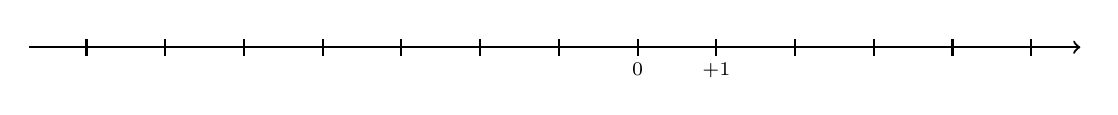
\begin{tikzpicture}

\begin{scope}[thick,font=\scriptsize]
  \draw[->] (-220pt,0)  - -  (160pt,0) node[above]{$\insZ$};	
    \foreach \n in {-7,-6,...,-1}{%
      \draw (\n,-3pt) -- (\n,3pt)   node [below=5pt] {};		
    }

    \foreach \m in {2,3,...,5}{%
      \draw (\m,-3pt) -- (\m,3pt) node [below=5pt]{};
    }

    \foreach \x in {1}{%
      \draw (\x,-3pt) -- (\x,3pt) node [below=5pt]{+$\x$};
    }
    
    \foreach \y in {0}{%
      \draw (\y,-3pt) -- (\y,3pt) node [below=5pt]{$\y$};
    }
\end{scope}
\end{tikzpicture}

\end{center}

\end{esercizio}

\begin{esercizio}
 \label{ese:2.3}
Per ciascuno dei seguenti numeri relativi scrivi il valore assoluto.
\begin{multicols}{3}
\begin{enumeratea}
 \item $|+3|=\ldots$;
 \item $|-5|=\ldots$;
 \item $|-1|=\ldots$;
 \item $|+10|=\ldots$;
 \item $|-11|=\ldots$;
 \item $|+7|=\ldots$
\end{enumeratea}
\end{multicols}
\end{esercizio}

 \begin{esercizio}
\label{ese:2.4}
Scrivi tra le seguenti coppie di numeri relativi il simbolo corretto tra ``$>$'' e ``$<$''.
\begin{multicols}{3}
 \begin{enumeratea}
 \item $ -5\ldots-2~$;
 \item $ -3\ldots+5~$;
 \item $ -2\ldots+2~$;
 \item $ -5\ldots0~$;
 \item $ -3\ldots-5~$;
 \item $ -1\ldots+1~$;
 \item $ +3\ldots-3~$;
 \item $ -1\ldots-5~$;
 \item $~0\ldots+1~$;
 \item $ +3\ldots0~$;
 \item $~0\ldots -2$;
 \item $ +7\ldots +2$;
 \item $ -11\ldots-101~$;
 \item $ +100\ldots-99~$;
 \item $ -101\ldots+110~$;
 \item $ -1\,010\ldots-1\,100~$;
 \item $ +324\ldots -282$;
 \item $ -714\ldots -851$.
 \end{enumeratea}
\end{multicols}
\end{esercizio}

\subsubsection*{2.4 - Le operazioni con i numeri relativi}

% % Addizione

\begin{esercizio}
 \label{ese:2.5}
Esegui le seguenti addizioni di numeri relativi.
 \begin{multicols}{3}
 \begin{enumeratea}
 \item $(+3)+(+2) =~$
 \item $(-5)+(-5) =~$
 \item $(-3)+(+5) =~$
 \item $(+12)+(+2) =$
 \item $(-2)+(-3) =$
 \item $(-3)+(+13) =$
 \item $(+10)+(-5) =$
 \item $(+1)+(+1) =$
 \item $(-10)+0 =$
 \item $(-4)+(+4) =$
 \item $(+7)+(-6) =$
 \item $(-9)+(-3) =$
 \item $(-101)+(+2) =$
 \item $0+(-9) =$
 \item $(-10)+(+10) =$
 \end{enumeratea}
 \end{multicols}
\end{esercizio}


\begin{esercizio}
 \label{ese:2.6}
Per ognuno dei seguenti numeri relativi scrivi il numero opposto.
 \begin{multicols}{3}
 \begin{enumeratea}
 \item $+3\to\ldots$;
 \item $-2\to\ldots$;
 \item $+1\to\ldots$;
 \item $-11\to\ldots$;
 \item $-3\to\ldots$;
 \item $+5 \to\ldots$
 \end{enumeratea}
 \end{multicols}
\end{esercizio}

\begin{esercizio}
 \label{ese:2.7}
Completa la seguente tabella.

 \begin{tabular*}{.9\textwidth}{@{\extracolsep{\fill}}*{11}{c}}
 \toprule
 $a$ &$+$1 &$-$2 &0 &$+$2 &$-$3 &$+$3 &$-$1 &$+$4 &$-$5 &$-$10\\
 $b$ &0 &$-$2 &$-$3&$+$1 &$-$5 &$-$3 &$-$10&$-$5 &$+$4 &$+$4 \\
 \midrule
 $a+b$& & &	& &	 & &	& &	 &\\
 \bottomrule
 \end{tabular*}

\end{esercizio}

% % Sottrazione
\pagebreak
\begin{esercizio}
Esegui le seguenti sottrazioni di numeri relativi.
\label{ese:2.8}
\begin{multicols}{3}
\begin{enumeratea}
 \item $(-1)-(+2) = \ldots$;
 \item $(-5)-(+3) = \ldots$;
 \item $(-2)-(+5) = \ldots$;
 \item $(+12)-(+2) = \ldots$;
 \item $(+1)-(-3) = \ldots$;
 \item $(-3)-(+1) = \ldots$;
 \item $(+11)-(-5) = \ldots$;
 \item $(+21)-(+11) = \ldots$;
 \item $(-1)-0 = \ldots$;
 \item $(-3)-(+4) = \ldots$;
 \item $(+7)-(-2) = \ldots$;
 \item $(-3)-(-3) = \ldots$;
 \item $0-(-11) = \ldots$;
 \item $(-6)-(-6) = \ldots$;
 \item $(+5)-(-5) = \ldots$
\end{enumeratea}
\end{multicols}
\end{esercizio}

\begin{esercizio}
 \label{ese:2.9}
Completa la seguente tabella.

 \begin{tabular*}{.9\textwidth}{@{\extracolsep{\fill}}*{11}{c}}
 \toprule
 $a$ &$-$2 &$-$2 &$-$3 &$+$2 &$-$10 &$+$3 &$-$1 &$-$7 &$+$8 &$-$9\\
 $b$ &0 &$-$3 &$-$3 &$-$5 &$-$5 &$-$1 &$-$10&$-$5 &$+$8 &$+$4 \\
 \midrule
 $a-b$& & &	& &	 & &	& &	 &\\
 \bottomrule
 \end{tabular*}

\end{esercizio}

\begin{esercizio}
 \label{ese:2.10}
Completa la seguente tabella.

 \begin{tabular*}{.9\textwidth}{@{\extracolsep{\fill}}*{11}{c}}
 \toprule
 $a$ &$-$2 &$+$2 &$-$1 &$+$2 &$-$10 &$-$5 &$-$1 &$-$7 &$+$8 &$-$9\\
 $b$ &$+$1 &$-$3 &$-$2 &$-$1 &$+$11 &$+$1 &$-$7 &$-$2 &$-$3 &$-$4 \\
 $c$ &$-$3 &$-$5 &$-$6 &$+$1 &$-$1	&$-$2 &$-$2 &$-$5 &$-$3 &$+$2\\
 \midrule
 $a-(b+c)$& & &	& &	 & &	& &	 &\\
 \bottomrule
 \end{tabular*}

\end{esercizio}

\begin{esercizio}
 \label{ese:2.11}
Completa la seguente tabella.

 \begin{tabular*}{.9\textwidth}{@{\extracolsep{\fill}}*{11}{c}}
 \toprule
 $a$ &$+$1 &$+$2 &$-$2 &$-$3 &$+$4 &$-$5 &$-$1 &$+$6 &$-$7 &$+$10\\
 $b$ &$-$1 &0 &$-$3 &$-$2 &$+$4 &$-$2 &$+$1 &$-$4 &$-$3 &$+$4\\
 $c$ &0	&$-$1 &$+$1 &$-$2 &$+$3 &$-$3 &$+$4 &$-$5 &$+$5 &$-$6\\
 \midrule
 $a-(b+c)$ & & & & & & & & & &\\
 \midrule
 $a-b+c$ & & & & & & & & & &\\
 \midrule
 $a-b-c$ & & & & & & & & & &\\
 \bottomrule
 \end{tabular*}
\end{esercizio}

\begin{esercizio}
 \label{ese:2.12}
Completa la seguente tabella.

 \begin{tabular*}{.9\textwidth}{@{\extracolsep{\fill}}*{11}{c}}
 \toprule
 $a$ &$-$2 &$+$2 &$-$1 &$+$1 &0 &$+$1 &$-$1 &$+$2 &$-$2 &$+$3\\
 $b$ &$-$1 &$+$1 &0 	 &$+$1 &$-$1 &$+$2 &$-$2 &$+$3 &$-$3 &$+$3\\
 \midrule
 $a+b$ & & & & & & & & & &\\
 \midrule
 $-a+b$ & & & & & & & & & &\\
 \midrule
 $-a-b$ & & & & & & & & & &\\
 \midrule
 $-(a+b)$ & & & & & & & & & &\\
 \midrule
 $-(a-b)$ & & & & & & & & & &\\
 \midrule
 $-(-a+b)$ & & & & & & & & & &\\
 \bottomrule
 \end{tabular*}
\end{esercizio}

% % Somma algebrica

\begin{esercizio}
Esegui le seguenti somme algebriche.
 \label{ese:2.13}
 \begin{multicols}{3}
 \begin{enumeratea}
 \item $+3 -1 = +\ldots$;
 \item $+2 -3 = -\ldots$;
 \item $-5 +2 = -\ldots$;
 \item $-2 +2 = \ldots\ldots$;
 \item $-5 -2 = \ldots7$;
 \item $-3 +5 = \ldots2$;
 \item $+8 -0 = \ldots\ldots$;
 \item $-9 +0 = \ldots\ldots$;
 \item $0 -5 = \ldots\ldots$;
 \item $+1 -1 = \ldots\ldots$;
 \item $-2 -2 = \ldots\ldots$;
 \item $+9 -3 = \ldots6$;
 \item $+7 -6 = +\ldots$;
 \item $-101 +9 = -\ldots$;
 \item $-10 +5 = \ldots~5$.
 \end{enumeratea}
 \end{multicols}
\end{esercizio}

\begin{esercizio}
 \label{ese:2.14}
Esegui le seguenti somme algebriche.
\begin{multicols}{3}
 \begin{enumeratea}
 \item $-5 -2 = \ldots$;
 \item $+3 -4 = \ldots$;
 \item $-1 +2 = \ldots$;
 \item $-3 +4 = \ldots$;
 \item $-6 +7 = \ldots$;
 \item $-1 -9 = \ldots$;
 \item $+8 -7 = \ldots$;
 \item $+2 -1 = \ldots$;
 \item $-6 +2 = \ldots$;
 \item $+5 -2 = \ldots$;
 \item $+4 -3 = \ldots$;
 \item $+4 +1 = \ldots$;
 \item $+4 -6 = \ldots$;
 \item $-10 +5 = \ldots$;
 \item $-16 -4 = \ldots$;
 \item $-3 -9 = \ldots$;
 \item $+14 -7 = \ldots$;
 \item $-10 -10 = \ldots$
 \end{enumeratea}

\end{multicols}

\end{esercizio}

% % Moltiplicazione
\begin{esercizio}
 \label{ese:2.15}
Calcola i seguenti prodotti.
\begin{multicols}{3}
 \begin{enumeratea}
 \item $(+3)\cdot(-2) =-\ldots$;
 \item $(-5)\cdot(-2)=+\ldots$;
 \item $(+2)\cdot(+4) =\ldots8$;
 \item $(+1)\cdot(-1) =\ldots1$;
 \item $(+3)\cdot0 = \ldots\ldots$;
 \item $(-2)\cdot(-2) =\ldots\ldots$;
 \item $0\cdot(-3) = \ldots\ldots$;
 \item $(-2)\cdot(+2) =\ldots\ldots$;
 \item $(+10)\cdot(-1) =\ldots\ldots$

 \end{enumeratea}
\end{multicols}
\end{esercizio}

\begin{esercizio}
 \label{ese:2.16}
Esegui le seguenti moltiplicazioni.
\begin{multicols}{3}
 \begin{enumeratea}
 \item $(+3)\cdot(+1) = \ldots$
 \item $(+1)\cdot(-2) = \ldots$;
 \item $(+3)\cdot(-3) = \ldots$;
 \item $(-5)\cdot(-1) = \ldots$;
 \item $(+3)\cdot(-3) = \ldots$;
 \item $(-2)\cdot(+5) = \ldots$;
 \item $(-1)\cdot(-7) = \ldots$;
 \item $(+3)\cdot(+11) = \ldots$;
 \item $(+1)\cdot(-10) = \ldots$;
 \item $(-4)\cdot(+3) = \ldots$;
 \item $(+5)\cdot(-6) = \ldots$;
 \item $(-3)\cdot(-2) = \ldots$
 \end{enumeratea}
\end{multicols}
\end{esercizio}

\begin{esercizio}
 \label{ese:2.17}
Completa la seguente tabella.

 \begin{tabular*}{.9\textwidth}{@{\extracolsep{\fill}}*{11}{c}}
 \toprule
$a$ &$-$2 &$+$2 &$-$1 &$+$2 &$-$10 &$-$5 &$-$1 &$-$7 &$+$8 &$-$9\\
 $b$ &$+$1 &$-$3 &$-$2 &$-$1 &$+$11 &$+$1 &$-$7 &$-$2 &$-$3 &$-$4 \\
 \midrule
$a\cdot b$& & &	& &	 & &	& &	 &\\
 \bottomrule
 \end{tabular*}

\end{esercizio}



% % Divisione
\begin{esercizio}
\label{ese:2.18}
 Esegui le seguenti divisioni.
\begin{multicols}{3}
 \begin{enumeratea}
 \item $(+4):(+2) = \ldots$;
 \item $(+5):(-1) = \ldots$;
 \item $(+6):(+2) = \ldots$;
 \item $(+8):(-2) = \ldots$;
 \item $(-8):(+4) = \ldots$;
 \item $(-4):(+2) = \ldots$;
 \item $(-10):(+5) = \ldots$;
 \item $(+10):(-2) = \ldots$;
 \item $(-12):(+6) = \ldots$;
 \item $(-12):(+4) = \ldots$;
 \item $(+12):(-3) = \ldots$;
 \item $(-12):(+1) = \ldots$
 \end{enumeratea}
 \end{multicols}
\end{esercizio}

\begin{esercizio}
 \label{ese:2.19}
Completa la seguente tabella.

 \begin{tabular*}{.9\textwidth}{@{\extracolsep{\fill}}*{11}{c}}
 \toprule
$a$ &$-$2 &$+$12 &$-$6 &$+$20 &$-$10 &$-$5 &$-$21 &$-$16 &$+$8 &$-$32\\
 $b$ &$+$1 &$-$3 &$-$2 &$-$1 &$-$5 &$+$1 &$-$7 &$-$2 &$-$4 &$-$4 \\
 \midrule
$a:b$& & &	& &	 & &	& &	 &\\
 \bottomrule
 \end{tabular*}

\end{esercizio}

\pagebreak
\begin{esercizio}
 \label{ese:2.20}
Completa la seguente tabella.

 \begin{tabular*}{.9\textwidth}{@{\extracolsep{\fill}}*{11}{c}}
 \toprule
 $a$ &0 &$+$2 &$+$1 &$-$4 &$-$6 &$-$8 &$+$10 &$+$12 &$-$14 &$-$16\\
 $b$ &$+$1 &$-$1 &$-$1 &$+$2 &$-$3 &$+$2 &$-$5 &$-$6 &$-$7 &$+$8\\
 \midrule
 $a:b$ & & & & & & & & & &\\
 \midrule
 $-a:b$ & & & & & & & & & &\\
 \midrule
 $-(a:b)$ & & & & & & & & & &\\
 \midrule
 $a:(-b)$ & & & & & & & & & &\\
 \bottomrule
 \end{tabular*}
\end{esercizio}

% % Potenza di un numero relativo
\begin{esercizio}
\label{ese:2.21}
Calcola il valore delle seguenti potenze.
\begin{multicols}{3}
 \begin{enumeratea}
 \item $(+3)^2 = \ldots$;
 \item $(-1)^2 = \ldots$;
 \item $(+1)^3 = \ldots$;
 \item $(-2)^2 = \ldots$;
 \item $(-2)^3 = \ldots$;
 \item $(+2)^3 = \ldots$;
 \item $(-3)^2 = \ldots$;
 \item $(-3)^3 = \ldots$;
 \item $(-4)^1 = \ldots$;
 \item $(+4)^1 = \ldots$;
 \item $(-4)^2 = \ldots$;
 \item $(-2)^4 = \ldots$;
 \item $(-3)^0 = \ldots$;
 \item $(-1)^5 = \ldots$;
 \item $(-2)^4 = \ldots$
 \end{enumeratea}
 \end{multicols}
\end{esercizio}

\begin{esercizio}
\label{ese:2.22}
 Applica le proprietà delle potenze.
\begin{multicols}{2}
 \begin{enumeratea}
 \item $(-3)^2\cdot(-3)^3 = (-3)^{\ldots}$;
 \item $(-2)^4\cdot(-2)^5 = (-2)^{\ldots}$;
 \item $(-5)\cdot(-5)^2 = (-5)^{\ldots}$;
 \item $(-10)^2\cdot(-5)^2 = (\ldots \ldots)^2$;
 \item $(-3)^4:(-3)^2 = (-3)^{\ldots}$;
 \item $(-7)^3:(-7)^3=(-7)^{\ldots}$;
 \item $(-2)^4:(-2)^2=(-2)^{\ldots}$;
 \item $(-6)^4:(+2)^4=(\ldots \ldots)^4$;
 \item $\big[(-3)^2\big]^3 = (-3)^{\ldots}$;
 \item $\big[(-5)^2\big]^3=(+5)^{\ldots}$;
 \item $(-3)^3\cdot(+3)^3 = \ldots$;
 \item $(-8)^2:(-4)^2= \ldots$;
 \item $\big[(-7)^2\big]^3: (-7)^3 =\ldots$;
 \item $\big[(-3)^3\big]^2: (-3)^4=\ldots$
 \end{enumeratea}
 \end{multicols}
\end{esercizio}


\begin{esercizio}
 \label{ese:2.23}
Completa la seguente tabella.

 \begin{tabular*}{.9\textwidth}{@{\extracolsep{\fill}}*{11}{c}}
 \toprule
 $a$ &$-$2 &$+$1 &$+$2 &$-$1 &$+$3 &$-$3 &$-$4 &$-$2 &$+$2 &$-$3\\
 $b$ &1 &3 &2 &4 &2 &3 &2 &4 &5 &2\\
 \midrule
 $a^b$ & & & & & & & & & &\\
 \bottomrule
 \end{tabular*}
\end{esercizio}


\begin{esercizio}
 \label{ese:2.24}
Completa la seguente tabella.

 \begin{tabular*}{.9\textwidth}{@{\extracolsep{\fill}}*{11}{c}}
 \toprule
~$a$ &$-$2 &$+$12 &$-$6 &$+$20 &$-$10 &$-$5 &$-$21 &$-$16 &$+$8 &$-$12\\
 $b$ &$+$1 &$-$3 &$-$2 &$-$1 &$-$5 &$+$1 &$+$19 &$-$14 &$-$4 &$-$8 \\
 \midrule
~$(a-b)^2$& & &	& &	 & &	& &	 &\\
 \bottomrule
 \end{tabular*}

\end{esercizio}

\begin{esercizio}
 \label{ese:2.25}
Completa la seguente tabella.

 \begin{tabular*}{.9\textwidth}{@{\extracolsep{\fill}}*{11}{c}}
 \toprule
~$a$ &$-$1 &$-$2 &$+$3 &0 &$+$1 &$+$2 &$-$4 &$+$5 &$-$5 &$-$3\\
 \midrule
~$a^2$& & &	& &	 & &	& &	 &\\
 \midrule
~$-a^2$& & &	& &	 & &	& &	 &\\
 \midrule
~$-(-a)^2$& & &	& &	 & &	& &	 &\\
 \bottomrule
 \end{tabular*}

\end{esercizio}

\begin{esercizio}
 \label{ese:2.26}
Completa la seguente tabella.

 \begin{tabular*}{.9\textwidth}{@{\extracolsep{\fill}}*{11}{c}}
 \toprule
$a$ &$-$2 &$-$3 &$+$3 &$-$1 &0 &$-$2 &$-$4 &$-$3 &$+$4 &$+$5\\
 $b$ &0 &$+$1 &$-$1 &$-$2 &$+$2 &$-$3 &$+$2 &$-$2 &$-$3 &$-$5\\
 \midrule
$a\cdot b$& & &	& &	 & &	& &	 &\\
 \midrule
$-a\cdot b$& & &	& &	 & &	& &	 &\\
 \midrule
$(-a)\cdot(-b)$& & &	& &	 & &	& &	 &\\
 \midrule
$-a^2	\cdot b$& & &	& &	 & &	& &	 &\\
 \bottomrule
 \end{tabular*}

\end{esercizio}

% % Proprietà distributiva della moltiplicazione rispetto all’addizione
\begin{esercizio}
 \label{ese:2.27}
Completa la seguente tabella.

 \begin{tabular*}{.9\textwidth}{@{\extracolsep{\fill}}*{11}{c}}
 \toprule
$a$ &$-$2 &$+$2 &$-$1 &$+$2 &$-$10 &$-$5 &$-$1 &$-$7 &$+$8 &$-$9\\
 $b$ &$+$1 &$-$3 &$-$2 &$-$1 &$+$11 &$+$1 &$-$7 &$-$2 &$-$3 &$-$4 \\
 $c$ &$-$3 &$-$5 &$-$6 &$+$1 &$-$1	&$-$2 &$-$2 &$-$5 &$-$3 &$+$2\\
 \midrule
$(a+b)\cdot c$& & &	& &	 & &	& &	 &\\
 \bottomrule
 \end{tabular*}

\end{esercizio}

\begin{esercizio}
 \label{ese:2.28}
Completa la seguente tabella.

 \begin{tabular*}{.9\textwidth}{@{\extracolsep{\fill}}*{11}{c}}
 \toprule
$a$ &$-$2 &$+$12 &$-$6 &$+$20 &$-$10 &$-$5 &$-$21 &$-$16 &$+$8 &$-$12\\
 $b$ &$+$1 &$-$3 &$-$2 &$-$1 &$-$5 &$+$1 &$+$19 &$-$14 &$-$4 &$-$8 \\
 \midrule
$(a+b)\cdot(a-b)$
 \end{tabular*}

\end{esercizio}

\begin{esercizio}
 \label{ese:2.29}
Completa la seguente tabella.

 \begin{tabular*}{.9\textwidth}{@{\extracolsep{\fill}}*{11}{c}}
 \toprule
$a$ &$+$1 &0 &$-$1 &$+$2 &$-$2 &0 &$+$3 &$-$3 &$+$4 &$-$10\\
 $b$ &$+$2 &0 &$+$1 &$-$1 &$-$2 &$-$3 &$+$2 &$+$3 &$+$4 &$+$8\\
 $c$ &$+$3 &$+$1 &$+$1 &$-$2 &$-$2 &$+$3 &$-$2 &0 &0 &$+$2\\
 \midrule
$-2\cdot a+(b-c)$& & &	& &	 & &	& &	 &\\
 \bottomrule
 \end{tabular*}

\end{esercizio}


\subsection{Esercizi riepilogativi}

\begin{esercizio}
In quali delle seguenti situazioni è utile ricorrere ai numeri relativi?
 \begin{enumeratea}
 \item misurare la temperatura;
 \item contare le persone;
 \item esprimere la data di nascita di un personaggio storico;
 \item esprimere l'età di un personaggio storico;
 \item indicare il saldo attivo o passivo del conto corrente;
 \item indicare l'altezza delle montagne e le profondità dei mari.
 \end{enumeratea}
\end{esercizio}

\begin{esercizio}
La somma di due numeri relativi è sicuramente positiva quando:
 \begin{multicols}{2}
 \noindent
 \usebox\boxa\: i due numeri sono concordi.\\
 \usebox\boxb\: i due numeri sono discordi.\\
 \usebox\boxc\: i due numeri sono entrambi positivi.\\
 \usebox\boxd\: i due numeri sono entrambi negativi.
 \end{multicols}
\end{esercizio}

\pagebreak
\begin{esercizio}
La somma di due numeri relativi è sicuramente negativa quando:
 \begin{multicols}{2}
 \noindent
 \usebox\boxa\: i due numeri sono concordi.\\
 \usebox\boxb\: i due numeri sono discordi.\\
 \usebox\boxc\: i due numeri sono entrambi positivi.\\
 \usebox\boxd\: i due numeri sono entrambi negativi.
 \end{multicols}
\end{esercizio}

\begin{esercizio}
Il prodotto di due numeri relativi è positivo quando (più di una risposta possibile):
 \begin{multicols}{2}
 \noindent
 \usebox\boxa\: i due numeri sono concordi.\\
 \usebox\boxb\: i due numeri sono discordi.\\
 \usebox\boxc\: i due numeri sono entrambi positivi.\\
 \usebox\boxd\: i due numeri sono entrambi negativi.
 \end{multicols}
\end{esercizio}

\begin{esercizio}
Il prodotto di due numeri relativi è negativo quando:
 \begin{multicols}{2}
 \noindent
 \usebox\boxa\: i due numeri sono concordi.\\
 \usebox\boxb\: i due numeri sono discordi.\\
 \usebox\boxc\: i due numeri sono entrambi positivi.\\
 \usebox\boxd\: i due numeri sono entrambi negativi.
 \end{multicols}
\end{esercizio}

\begin{esercizio}
Quali delle seguenti affermazioni sono vere?
\TabPositions{12cm}
\begin{enumeratea}
 \item ogni numero relativo è minore di zero \tab\boxV\quad\boxF
 \item la somma di due numeri discordi è zero \tab\boxV\quad\boxF
 \item il cubo di un numero intero relativo è sempre negativo \tab\boxV\quad\boxF
 \item la somma di due numeri opposti è nulla \tab\boxV\quad\boxF
 \item il quoziente di due numeri opposti è l'unità \tab\boxV\quad\boxF
 \item il quoziente di due numeri concordi è positivo \tab\boxV\quad\boxF
 \item il prodotto di due numeri opposti è uguale al loro quadrato \tab\boxV\quad\boxF
 \item il doppio di un numero intero negativo è positivo \tab\boxV\quad\boxF
 \item la somma di due interi concordi è sempre maggiore di ciascun addendo \tab\boxV\quad\boxF
 \item il quadrato dell'opposto di un intero è uguale all'opposto del suo quadrato \tab\boxV\quad\boxF
\end{enumeratea}
\end{esercizio}

\begin{esercizio}
Inserisci l'operazione corretta per ottenere il risultato.
 \begin{multicols}{3}
 \begin{enumeratea}
 \item $(+2)\ldots(-1) = -2$;
 \item $(-10)\ldots(+5) = -2$;
 \item $(-18)\ldots(-19) = +1$;
 \item $(+15)\ldots(-20) = -5$;
 \item $(-12)\ldots(+4) = -3$;
 \item $(-4)\ldots0 =~0$;
 \item $(+1)\ldots(+1) =~0$;
 \item $(+5)\ldots(-6) = +11$;
 \item $-8\ldots(-2) = +16$.
 \end{enumeratea}
 \end{multicols}
\end{esercizio}


\begin{esercizio}
Inserisci il numero mancante.
 \begin{multicols}{3}
 \begin{enumeratea}
 \item $+5 + (\ldots\ldots) = -5$;
 \item $-8 + (\ldots\ldots) = -6$;
 \item $+7 - (\ldots\ldots) =~0$;
 \item $0 - (\ldots\ldots) = -2$;
 \item $+3\cdot (\ldots\ldots) = -3$;
 \item $-5\cdot (\ldots\ldots) =~0$;
 \item $(+16): (\ldots\ldots) = -2$;
 \item $(-6): (\ldots\ldots) = -1$;
 \item $(-10): (\ldots\ldots) = +5$.
 \end{enumeratea}
 \end{multicols}
\end{esercizio}

\begin{esercizio}
 Scrivi tutti i numeri:
 \begin{enumeratea}
 \item interi relativi che hanno valore assoluto minore di~5;
 \item interi relativi il cui prodotto è~$-$12;
 \item interi negativi maggiori di~$-$5.
 \end{enumeratea}
\end{esercizio}

\begin{esercizio}
Inserisci ``$+$'' o ``$-$'' in modo da ottenere il numero più grande possibile:
 \[-3\ldots(-3)\ldots3\ldots(-6).\]
\end{esercizio}

\begin{esercizio}[\Ast]
Inserisci le parentesi in modo da ottenere il risultato indicato.
 \begin{enumeratea}
 \item $-5 \cdot +3-1+2=-20$;
 \item $-5+2\cdot-1+2=+5$;
 \item $-5+7-3\cdot 2=+3$;
 \item $-1\cdot +3-5\cdot -1-2=+12$;
 \item $+1-1\cdot 1 -1+3-2\cdot -3-2=+5$.
 \end{enumeratea}
\end{esercizio}

\begin{esercizio}[\Ast]
Calcola il valore delle seguenti espressioni.
 \begin{enumeratea}
 \item $-5+7+4-9$;
 \item $+1-1+1-1+1-1+1$;
 \item $+1-2+3-4+5-6$;
 \item $+1-2+2-3+3-4+5-6+6-7+7-8+8-9+9-10$;
 \item $(-3+10)-(2-3)$.
 \end{enumeratea}
\end{esercizio}

\begin{esercizio}[\Ast]
Calcola il valore delle seguenti espressioni.
 \begin{enumeratea}
 \item $(+5-2-1)+(+2+4+6)$;
 \item $(-5+7-9)+(+1-2+3)-(+4-6+8)$;
 \item $+4-3-[+2-1-(8-3)-(-5-2)]-(2+3)$;
 \item $-2+(-5+1)+(-7+4)-2 \cdot (-6+1)$;
 \item $15-9 \cdot (-14+12)+8 \cdot (-3+6)+ 5 \cdot(-3+1)$.
 \end{enumeratea}
\end{esercizio}

\begin{esercizio}[\Ast]
Calcola il valore delle seguenti espressioni.
 \begin{enumeratea}
 \item $(50-36-25)\cdot (-15+5+20)-10\cdot (-3-7)$;
 \item $[+3-(10-5+25)]\cdot [-16+5-(-2-14)]:(9+6)$;
 \item $20:(+15-5)-30:(-10+5)+40:(15-20)$;
 \item $18:(-3)+6\cdot [1-5\cdot (-2+4)+3]: (-6)$;
 \item $3\cdot 4-3\cdot \left[18:\left(-2\right)-17+\left(14-26+5\right)\cdot 3-12\right]+\left[16-1\cdot \left(-1-3+5\right)-37+16\right]$.
\end{enumeratea}
\end{esercizio}

\begin{esercizio}[\Ast]
Calcola il valore delle seguenti espressioni e indica dove puoi applicare le proprietà delle potenze.
\TabPositions{3.5cm}
\begin{enumeratea}
 \item $100:2+3^2 -2^2\cdot 6$ \tab Hai applicato le proprietà delle potenze?\:\dotfill
 \item $2^7:~2^3 -2^2$ \tab Hai applicato le proprietà delle potenze?\:\dotfill
 \item $30-5\cdot 3 -7\cdot 2^2 -2$ \tab Hai applicato le proprietà delle potenze?\:\dotfill
 \item $\left(3^2 +4^2\right) -(-3-4)^2$ \tab Hai applicato le proprietà delle potenze?\:\dotfill
\end{enumeratea}
\end{esercizio}

\begin{esercizio}[\Ast]
Calcola il valore delle seguenti espressioni e indica dove puoi applicare le proprietà delle potenze.
\TabPositions{5.5cm}
\begin{enumeratea}
 \item $5\cdot 5^3\cdot 5^4: \big(5^2\big)^3 +5$ \tab Hai applicato le proprietà delle potenze?\:\dotfill
 \item $32^5:~16^4 +(-2)^9$ \tab Hai applicato le proprietà delle potenze?\:\dotfill
 \item $\big(3^4\cdot 3^3:~3^6\big)^2 +\left(7^2-5^2\right):2^2$ \tab Hai applicato le proprietà delle potenze?\:\dotfill
 \item $\big(3\cdot 2^2 -10\big)^4\cdot \left(3^3+2^3\right):7-10\cdot 2^3$ \tab Hai applicato le proprietà delle potenze?\:\dotfill
\end{enumeratea}
\end{esercizio}

\begin{esercizio}[\Ast]
Calcola il valore delle seguenti espressioni.
 \begin{enumeratea}
 \item $-5\cdot(12-3+4)-2\cdot\left[3-16:(-2+4)\right]^2$;
 \item $\left[-3+(-5)\cdot(-1)\right]^3+\left[-4-(1-2)\right]^2$;
 \item $\left[2\cdot(-3)^2+2\cdot(-3)\cdot(-2)\right]^2:\left[2^4-3\cdot(+6)\right]^2$;
 \item $\left[3\cdot(-1)^2-3\cdot(-3)\cdot(-3)\right]^3:\left[2^2+5\cdot(-2)^2\right]^3$.
 \end{enumeratea}
\end{esercizio}

\begin{esercizio}[\Ast]
Calcola il valore delle seguenti espressioni.
 \begin{enumeratea}
 \item $(-3)^2\cdot(4-1)^5:\left[(-4)^3:\left(2^5\right)-3^3:(-3)^3\right]$;
 \item $\left[-(-2)\cdot2+(-10)^2:(-5)^2\right]\cdot\left[3-5+2\cdot(-3)^2-5\right]$;
 \item $13-3-4\cdot(-2)^2-5^3:5^2+3\cdot\left(2^3-3^2\right)-6:(-3)-(4-7+3)^4$;
 \item $-1-3\cdot(-3)^2-4^3:4^2+(-3-3)\cdot\left(2^2+3^2\right)-(-12):(-3)$.
 \end{enumeratea}
\end{esercizio}

\begin{esercizio}[\Ast]
Calcola il valore delle seguenti espressioni.
 \begin{enumeratea}
 \item $\left[10-6\cdot(-2)^2\right]:(-7)+\left(3^2:3\right)\cdot2^3-15:(-3)+\left[(-3)^3:(-3)^0\right]$;
 \item $|-5+8|-|-11|+(-|+4|\cdot|-2\cdot(+5)|)^2$;
 \item $(-29+37)^5\cdot(-5+|23-28|)^7$;
 \item $-2\cdot(-2\cdot|-2|)^2-(|3-5|\cdot(3-5))^2\cdot(-2)$;
 \item $(-1)^3\cdot(-1\cdot|-1|)^2-(|-3-2|\cdot(-5+3))^2\cdot(-2+1)^3$.
 \end{enumeratea}
\end{esercizio}
\begin{multicols}{2}
\begin{esercizio}
Traduci in una espressione matematica le seguenti frasi e motivane la verità o falsità:
 \begin{enumeratea}
 \item il cubo del quadrato di un numero diverso da zero è sempre positivo;
 \item il quadrato della somma di un numero con il suo opposto è sempre positivo;
 \item la differenza tra il triplo di~5 e l'unità è uguale all'opposto di~5;
 \item il prodotto tra il quadrato di un numero negativo e l'opposto dello stesso numero è uguale all'opposto del suo cubo.
 \end{enumeratea}
\end{esercizio}

\begin{esercizio}
 Sottrarre dal cubo di~$-3$ la somma dei quadrati di~$+2$ e~$-2$. Il risultato è?
\end{esercizio}

\begin{esercizio}
 Sottrarre dalla somma di~$-15$ e~$+27$ il prodotto di~$-3$ e~$+7$.
\end{esercizio}

\begin{esercizio}
 Aggiungere al prodotto di~$-5$ e~$+3$ la somma di~$+5$ e~$-10$.
\end{esercizio}

\begin{esercizio}
 Sottrarre dal prodotto di~$+7$ e~$+4$ la somma di~$+1$ e~$-8$.
\end{esercizio}

\begin{esercizio}
 Moltiplica la somma tra~$-3$ e~$+3$ con la differenza tra~$+3$ e~$-3$.
\end{esercizio}

\begin{esercizio}
 Partendo dal pian terreno scendo di~15 gradini, salgo~12 gradini, scendo di~7
gradini e risalgo di~8. A che punto mi trovo rispetto al pian terreno?
\end{esercizio}

\begin{esercizio}[\Ast]
 Giocando a carte contro due avversari nella prima partita ho vinto~50 gettoni con il primo giocatore e perso~60
gettoni con il secondo giocatore, nella seconda partita ho perso~30 gettoni con il primo e vinto~10 gettoni
con il secondo. Quanti gettoni ho vinto o perso complessivamente?

Se il primo giocatore deve dare 30~gettoni al secondo, chiedo al primo di dare al secondo anche i gettoni che doveva a me. Quanto darà il primo al secondo giocatore? Quanto dovrò dare io al secondo giocatore per chiudere tutti i conti della partita?
\end{esercizio}

\begin{esercizio}[\Ast]
 Un polpo congelato è stato appena tolto dal congelatore, la sua temperatura è~$-12\grado$C;
viene immerso nell'acqua bollente e la sua temperatura media è aumentata di~$6\grado$C.
A quale temperatura media si trova ora il polpo?
\end{esercizio}

\begin{esercizio}
 Una lumaca sale su un muro alto~10 metri, di giorno sale di due metri ma di notte
scende di un metro. In quanti giorni la lumaca arriva in cima al muro?
\end{esercizio}

\begin{esercizio}[\Ast]
 Un termometro segna all'inizio~$-5\grado$C, poi scende di~$3\grado$C, quindi sale di~$2\grado$C,
infine discende di~$6\grado$C. Quale temperatura segna alla fine?
\end{esercizio}

\begin{esercizio}[\Ast]
 Il prodotto di due numeri interi relativi è~$+80$, aumentando di~1 il primo numero il
prodotto è~$+72$. Quali sono i due numeri?									
\end{esercizio}

\begin{esercizio}
 Il prodotto di due numeri interi relativi è~$+6$, la loro somma è~$-5$. Quali sono i due numeri?
\end{esercizio}


\begin{esercizio}
 Determina due numeri relativi aventi come prodotto~$+12$ e come somma~$-7$.
\end{esercizio}

\begin{esercizio}
 Determina due numeri relativi aventi come
prodotto~$+12$ e come somma~$-7$.
\end{esercizio}

\begin{esercizio}
 Determina due numeri relativi aventi come
prodotto~$+2$ e come somma~$+1$.
\end{esercizio}

\begin{esercizio}
 Determina due numeri relativi aventi come
prodotto~$+10$ e come somma~$-3$.
\end{esercizio}

\begin{esercizio}
 Determina due numeri relativi aventi come
prodotto~$+14$ e come somma~$-9$.
\end{esercizio}

\begin{esercizio}
 Determina due numeri relativi aventi come
prodotto~$-15$ e come somma~$-8$.
\end{esercizio}

\begin{esercizio}
 Determina due numeri relativi aventi come
prodotto~$-7$ e come somma~$+6$.
\end{esercizio}
\end{multicols}
\subsection{Risposte}

\paragraph{2.40.}
a)~$-5\cdot(+3-1+2)$,\quad b)~$(-5+2)\cdot(-1)+2$,\quad c)~$-5+(7-3)\cdot2$.

\paragraph{2.41.}
a)~$-3$,\quad b)~$+1$,\quad c)~$-3$,\quad d)~$-8$,\quad e)~$+8$.

\paragraph{2.42.}
a)~$+14$,\quad b)~$-11$,\quad c)~$-7$,\quad d)~$+1$,\quad e)~$+47$.

\paragraph{2.43.}
a)~$-10$,\quad b)~$-9$,\quad c)~$0$,\quad d)~$0$,\quad e)~$+183$.

\paragraph{2.44.}
a)~$+35$,\quad b)~$+12$,\quad c)~$-15$,\quad d)~$-24$.

\paragraph{2.45.}
a)~$+30$,\quad b)~$0$,\quad c)~$+15$,\quad d)~$0$.

\paragraph{2.46.}
a)~$-115$,\quad b)~$+17$,\quad c)~$+225$,\quad d)~$-1$.

\paragraph{2.47.}
a)~$-3^7$,\quad b)~$+88$,\quad c)~$-12$,\quad d)~$-114$.

\paragraph{2.48.}
a)~$+4$,\quad b)~$+\np{1592}$,\quad c)~$0$,\quad d)~$0$.

\paragraph{2.56.}
Ho perso 30~gettoni, il primo deve dare~50 al secondo e io devo dare~30 al secondo.

\paragraph{2.59.}
$-6$\textdegree.

\paragraph{2.60.}
$-10$; $-8$.

\cleardoublepage
